\documentclass{article}
\usepackage[utf8]{inputenc}
\usepackage{amssymb}
\usepackage{color}
\usepackage{amsmath}
\usepackage{Sweave}
\usepackage{enumerate}
\usepackage{hyperref}
\usepackage{graphicx}

% \usepackage{subfig}
\graphicspath{ {./images/} }
\usepackage[margin=0.5in]{geometry}
\usepackage{gensymb}
\usepackage{textcomp}
\usepackage{siunitx}
\usepackage{wrapfig}
\usepackage{lipsum}
\usepackage{float}
\usepackage{hyperref}

\usepackage{amsmath}
\title{Projekt Zaliczeniowy z przedmiotu Rownania Rozniczkowe i Roznicowe}
\author{\textbf{404838, Dzmitry Mikialevich}, sroda $12^{50}$\\
\textit{AGH, Wydzial Informatyki Elektroniki i Telekomunikacji}\\
\date{Krakow, \today}
}
\begin{document}
\Sconcordance{concordance:Report.tex:Report.Rnw:%
1 110 1 1 2 4 0 1 2 1 1 1 20 22 0 1 2 2 1 1 10 1 2 5 1 1 23 24 0 1 2 1 %
1 1 12 14 0 1 2 2 1 1 13 15 0 1 2 2 1 1 4 6 0 1 2 1 18 17 0 1 8 8 0 1 2 %
2 1 1 20 22 0 1 2 2 1 1 8 10 0 1 2 2 1 1 2 8 0 1 2 5 1 1 25 24 0 2 1 3 %
0 2 2 23 0 1 2 2 1 1 2 1 0 1 1 4 0 1 2 9 1}

\maketitle
\tableofcontents
\newenvironment{centerfig}
{\begin{figure}[H]\centering}
{\end{figure}}
\newpage

\section{Zadanie}

\begin{equation*}
 \begin{cases}
   - \frac{d}{dx}(E(x)\frac{du(x)}{dx}) = 0 \\
   u(2) = 0 \\
   \frac{du(0)}{dx} + u(0) = 10
 \end{cases}
\end{equation*}


\begin{equation*}
  E(x) = 
  \begin{cases}
    3\: dla\: x \in [0,1] \\
    5\: dla\: x \in  (1,2]\\
  \end{cases}
 \end{equation*}

 \begin{equation*}
x \in [0,2]
 \end{equation*}


\section{Rozwiazanie}

\subsection{Sformulowanie Warjacyjne}


\[-(E(x)u'(x))' = 0 \Rightarrow -E'(x)u'(x) - u''(x)E(x)=0  \Rightarrow\]
Niech \(v: [0,2] -> \mathbb{R}\)
\[-\int_0^2{vE'(x)u'(x)dx} - \int_0^2{vu''(x)E(x)dx} = 0\Rightarrow\]
      
 \[E(x)v(x)u'(x) |_0^2 -  \int_0^2{y'(x)v'(x)E(x)dx}=0\]
\[E(2)v(2)u'(2) - E(0)v(0)u'(0) - \int_0^2{u'(x)v'(x)E(x)} = 0 \]  
Wiedzac, ze \(u'(0) = 10-u(0)\) i \(u(2)=0\):
\[\int_0^2{u'(x)v'(x)E(x)dx} = -10 E(0)v(0) + E(0)v(0)u(0)\]

\[\int_0^2{u'(x)v'(x)E(x)dx} - 3v(0)u(0)= -30 v(0)\]

\begin{equation*}
  \begin{cases}
B(u,v) =\int_0^2{u'(x)v'(x)E(x)dx} - 3v(0)u(0) \\
 L(v) =  -30 v(0) \\
  \end{cases}
\end{equation*}

\subsection{Metoda Galerkina}
\begin{equation*}
\begin{bmatrix}B(e_0,e_0) & & & & & B(e_{n-1},e_0) & | & B(e_n,e_0) \\\vdots & \ddots & & & & \vdots & | &\vdots \\\vdots & & & \ddots & & \vdots & | &\vdots \\\vdots & & & & \ddots & \vdots & | &\vdots \\ B(e_{n-1},e_0) & & & & & B(e_{n-1},e_{n-1}) & | & B(e_n,e_{n-1}) \\- - - & - - - & - - - & - - - & - - - & - - - & | & - - - \\& & & 0 & & B(e_{n-1},e_n) & | & B(e_{n},e_n)\end{bmatrix}\begin{bmatrix}u_0 \\u_1 \\\vdots \\\vdots \\\vdots \\u_{n-1} \\\\u_n \end{bmatrix}\begin{bmatrix}L(e_0) \\L(e_1) \\\vdots \\\vdots \\\vdots \\L(e_{n-1}) \\\\L(e_n) \end{bmatrix}
\end{equation*}

Majac nieskonczony wymiar \(V\), konstruujemy ciag \(V_n \subset V\), oraz wybieramy wektory bazowe ksztaltu:

\begin{equation*}
  e_i(x) = 
  \begin{cases}
  1 - |\frac{n}{2} (x - \frac{2i}{n})|\:,\: dla\: 1 - |\frac{n}{2} (x - \frac{2i}{n})|>=0 \\
  0\:, \: wpp \\
  \end{cases}
\end{equation*}


Oraz pochodna wektora bazowego:
\begin{equation*}
  e_i'(x) = 
  \begin{cases}
  \frac{n}{2}\:,\: dla\: x \in [\frac{2(i-1)}{n},\frac{2i}{n})\\
  -\frac{n}{2}\:,\: dla\: x \in [\frac{2i}{n},\frac{2(i+1)}{n})\\
  0\:, \: wpp \\
  \end{cases}
\end{equation*}

\section{Czesc numeryczna}
\subsection{Inicjalizacja projektu i stalych}
\begin{Schunk}
\begin{Sinput}
> library(cubature)
\end{Sinput}
\end{Schunk}

\subsection{Definicja Wektoru Bazowego:}
\begin{Schunk}
\begin{Sinput}
> e <- function(n,i){
+   return (
+     
+     Vectorize(
+       function(x){
+         tmp_n <- n/2
+         if (1 - abs(tmp_n * (x - i / tmp_n)) >= 0){
+           return (1 - abs(tmp_n * (x - i / tmp_n)))
+         }
+         else{
+           return (0)
+         }
+         
+         
+       }
+     )
+     
+   )
+ }
\end{Sinput}
\end{Schunk}
\subsection{Badanie wykresu \(e_i\) Na przykladzie \(n=4\)}

\begin{centerfig}
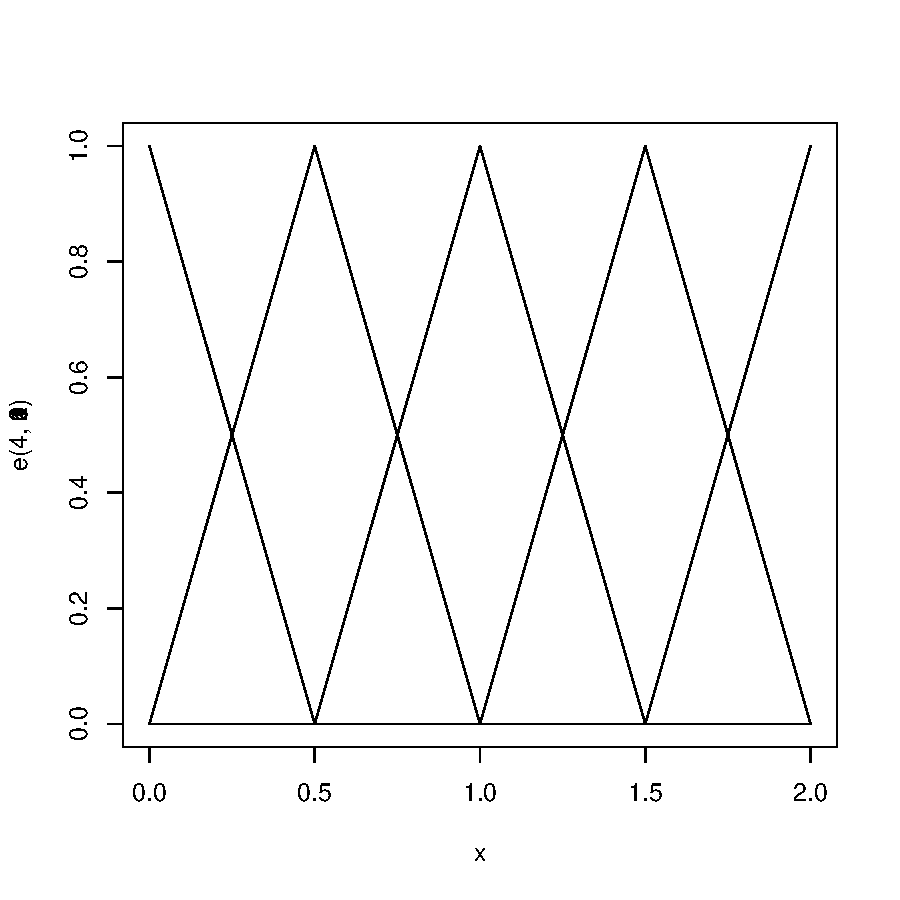
\includegraphics{Report-003}
\caption{Wykresy \(e_i\) dla n=4}
\end{centerfig}


\subsection{Definicja pochodnej Wektoru Bazowego:}

\begin{Schunk}
\begin{Sinput}
> e_prim <- function(n,i){
+   return (
+     
+     Vectorize(
+       function(x){
+         tmp_n <- n/2
+         if ((i - 1) / tmp_n <= x  && x< (i / tmp_n)){
+           return (tmp_n)
+         }
+         else if (i / tmp_n <= x && x< (i + 1) / tmp_n){
+           return (-tmp_n)
+         }
+         else{
+           return (0)
+         }
+         
+       }
+     )
+     
+   )
+ }
\end{Sinput}
\end{Schunk}

\subsection{Definicja \(E(x)\)}
\begin{Schunk}
\begin{Sinput}
> E <- function(x){
+   if (x<=1 && x>=0){
+     return (3)
+   }  
+   else if (x>1 && x<=2){
+     return (5)
+   }
+   else {
+     return (0)
+   }
+ }
\end{Sinput}
\end{Schunk}

\subsection{Definicja \(B(e_i,e_j)\)}

\begin{Schunk}
\begin{Sinput}
> B <- function(i,j,n){
+   h<- 2/n
+   return (
+     cubintegrate(
+       function(x){
+         return (e_prim(n,i)(x) * e_prim(n,j)(x) * (E(x)))
+       },
+       max(0,i*h-h),min(2,i*h+h),method="hcubature"
+       
+     )$integral - (3 * e(n,i)(0) * e(n,j)(0))     
+   )
+ }
\end{Sinput}
\end{Schunk}

\subsection{Definicja \(L(e_i)\)}

\begin{Schunk}
\begin{Sinput}
> L <- function(i,n){
+   return (-10 * E(0) * e(n,i)(0))
+ }
\end{Sinput}
\end{Schunk}
\subsection{Budowanie macierzy B i L}
\begin{Schunk}
\begin{Sinput}
> Build_B_M <- function(n){
+ 
+ B_M <- matrix(nrow=n-1,ncol = n-1)
+ 
+ for (i in 1:(n-1))
+   for (j in 1:(n-1)){
+     if (abs(i-j)<=1){
+       B_M[i,j] <- B(i-1,j-1,n)
+     }
+     else{
+       B_M[i,j] = 0
+     }
+     
+   }
+   return (B_M)
+ 
+ }
> Build_L_M <- function(n){
+   L_M <- matrix(nrow=n-1,ncol = 1)
+   for (i in 1:(n-1))
+     L_M[i] <- L(i-1,n)
+   return (L_M)
+ }
\end{Sinput}
\end{Schunk}

\subsection{Rysowanie wyniku w postaci punktowej}

\begin{Schunk}
\begin{Sinput}
> draw_results <- function(points,n,u_v){
+ x_v = c()
+ y_v = c()
+ 
+ for (curr in 1:points){
+   
+   x <- curr*2/points
+   y <- 0
+   for (v in 1:length(u_v)){
+     y = y + u_v[v]*e(n,v-1)(x)
+   }
+   
+   x_v = append(x_v,x)
+   y_v = append(y_v,y)
+ 
+   
+ }
+  plot(x_v,y_v)
+ }
\end{Sinput}
\end{Schunk}


\subsection{Zbieranie wszystkiego w jedna funkcje}
\begin{Schunk}
\begin{Sinput}
> solve_equation <- function(n,points){
+   B_M <- Build_B_M(n)
+   L_M <- Build_L_M(n)
+   u_v <- solve(B_M,L_M)
+   draw_results(points,n,u_v)
+   print(n)
+ }
\end{Sinput}
\end{Schunk}

\subsection{Sprawdzenie dzialania}
\begin{centerfig}
\begin{Schunk}
\begin{Sinput}
> solve_equation(100,100)
\end{Sinput}
\begin{Soutput}
[1] 100
\end{Soutput}
\end{Schunk}
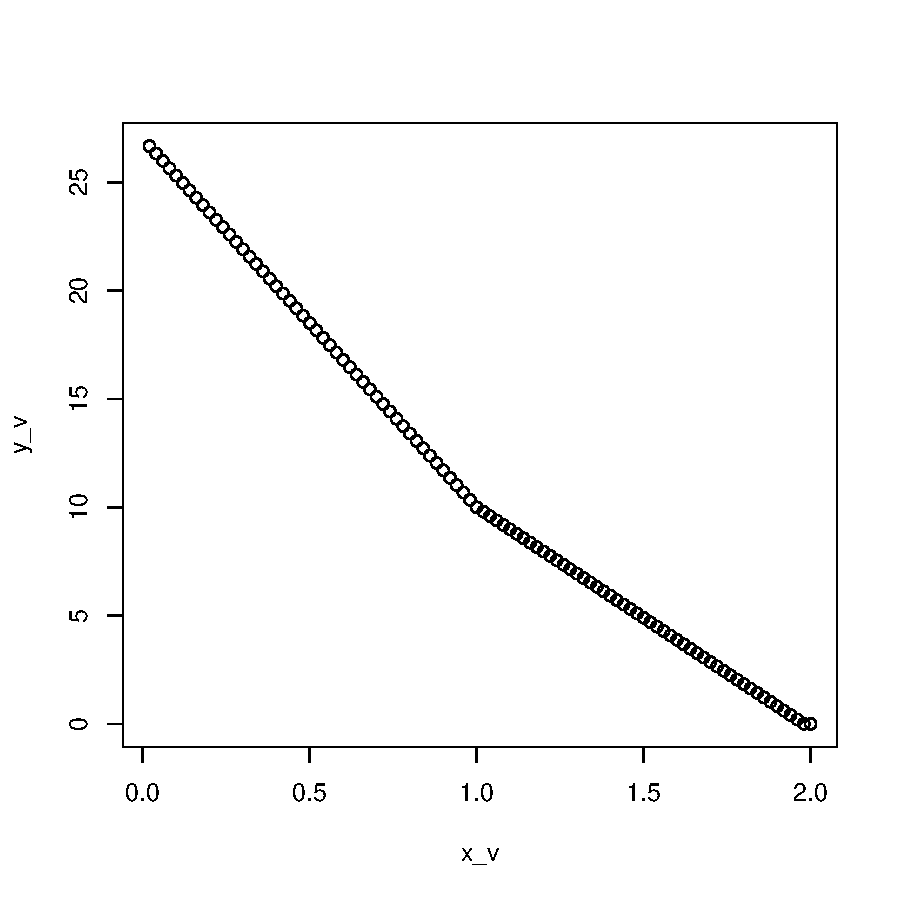
\includegraphics{Report-011}
\caption{Solution plot}
\end{centerfig}

\section{Budowanie modelu dla badania rownania prosej}


\begin{Schunk}
\begin{Sinput}
> build_model <- function(n,points){
+   B_M <- Build_B_M(n)
+   L_M <- Build_L_M(n)
+   u_v <- solve(B_M,L_M)
+   x_v = c()
+   y_v = c()
+   for (curr in 1:points){
+     
+     x <- curr*2/points
+     y <- 0
+     
+     for (v in 1:length(u_v)){
+       y = y + u_v[v]*e(n,v-1)(x)
+     }
+     
+     x_v = append(x_v,x)
+     y_v = append(y_v,y)
+   
+     
+   }
+   frame <- data.frame(x_v,y_v)
+  
+   return (frame)
+ }
> frame <- build_model(150,100)
> model <- lm(frame$y_v ~ frame$x_v)
\end{Sinput}
\end{Schunk}

\begin{Schunk}
\begin{Sinput}
> summary(model)
\end{Sinput}
\begin{Soutput}
Call:
lm(formula = frame$y_v ~ frame$x_v)

Residuals:
    Min      1Q  Median      3Q     Max 
-1.6900 -0.8359 -0.0008  0.8396  1.7688 

Coefficients:
            Estimate Std. Error t value Pr(>|t|)    
(Intercept)   25.149      0.199  126.38   <2e-16 ***
frame$x_v    -13.459      0.171  -78.69   <2e-16 ***
---
Signif. codes:  0 '***' 0.001 '**' 0.01 '*' 0.05 '.' 0.1 ' ' 1

Residual standard error: 0.9875 on 98 degrees of freedom
Multiple R-squared:  0.9844,	Adjusted R-squared:  0.9843 
F-statistic:  6191 on 1 and 98 DF,  p-value: < 2.2e-16
\end{Soutput}
\end{Schunk}


\begin{centerfig}
\begin{Schunk}
\begin{Sinput}
> plot(frame)
> abline(model)
\end{Sinput}
\end{Schunk}
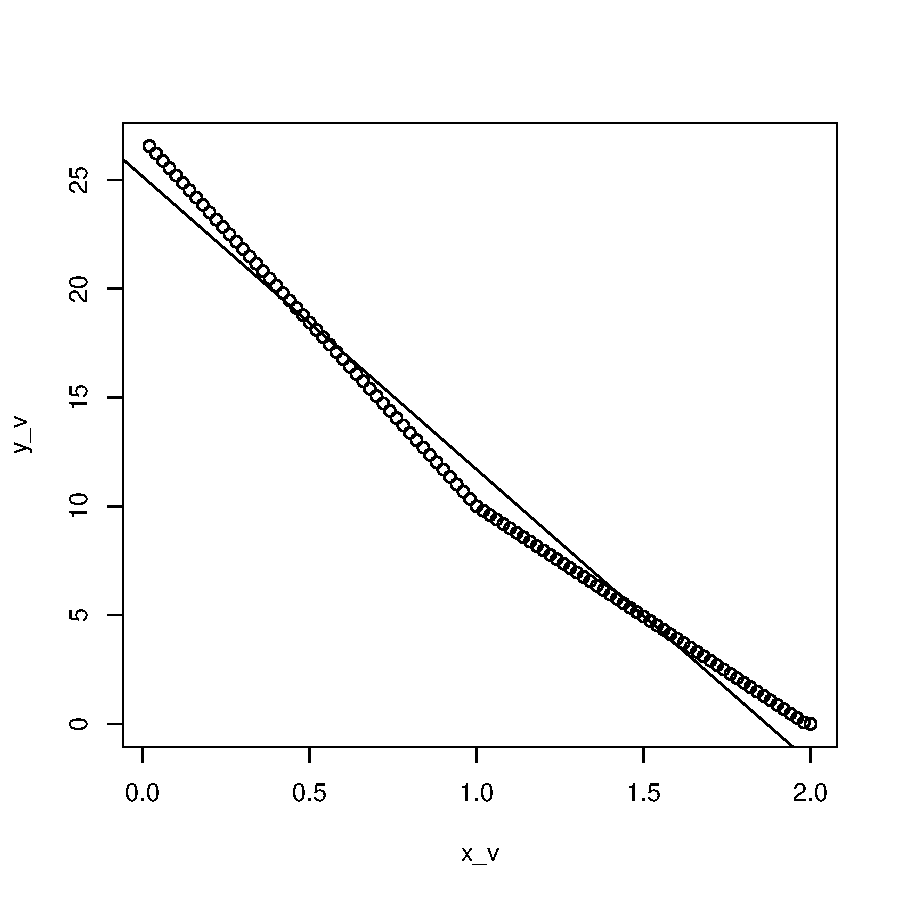
\includegraphics{Report-014}
\caption{Ablined Model}
\end{centerfig}


\section{Postac Rownania}
\[y = -13.4x + 25.1\]

\end{document}


